\subsection{Charakterisierung des Pr:YLF-Kristalls}

\subsubsection{Absorptionsspektrum}

Zur Bestimmung des Absorptionsspektrums des Pr:YLF-Kristalls wurde mit dem USB-Spektrometer ein
Referenzspektrum aufgezeichnet (Tageslicht vom Himmel), dann das Transmissionsspektrum des Kristalls
mit dem gleichen Licht aufgezeichnet und (vom Spektrometer) das Absorptionsspektrum als Differenz
berechnet.
Abb.~\ref{img:AbsSpec} zeigt das berechnete Spektrum.
Die Lage der Absorptionsmaxima ist eingezeichnet und in Tab.~ \ref{tab:AbsSpec} aufgeführt.

\begin{figure}[H]
\begin{center}
  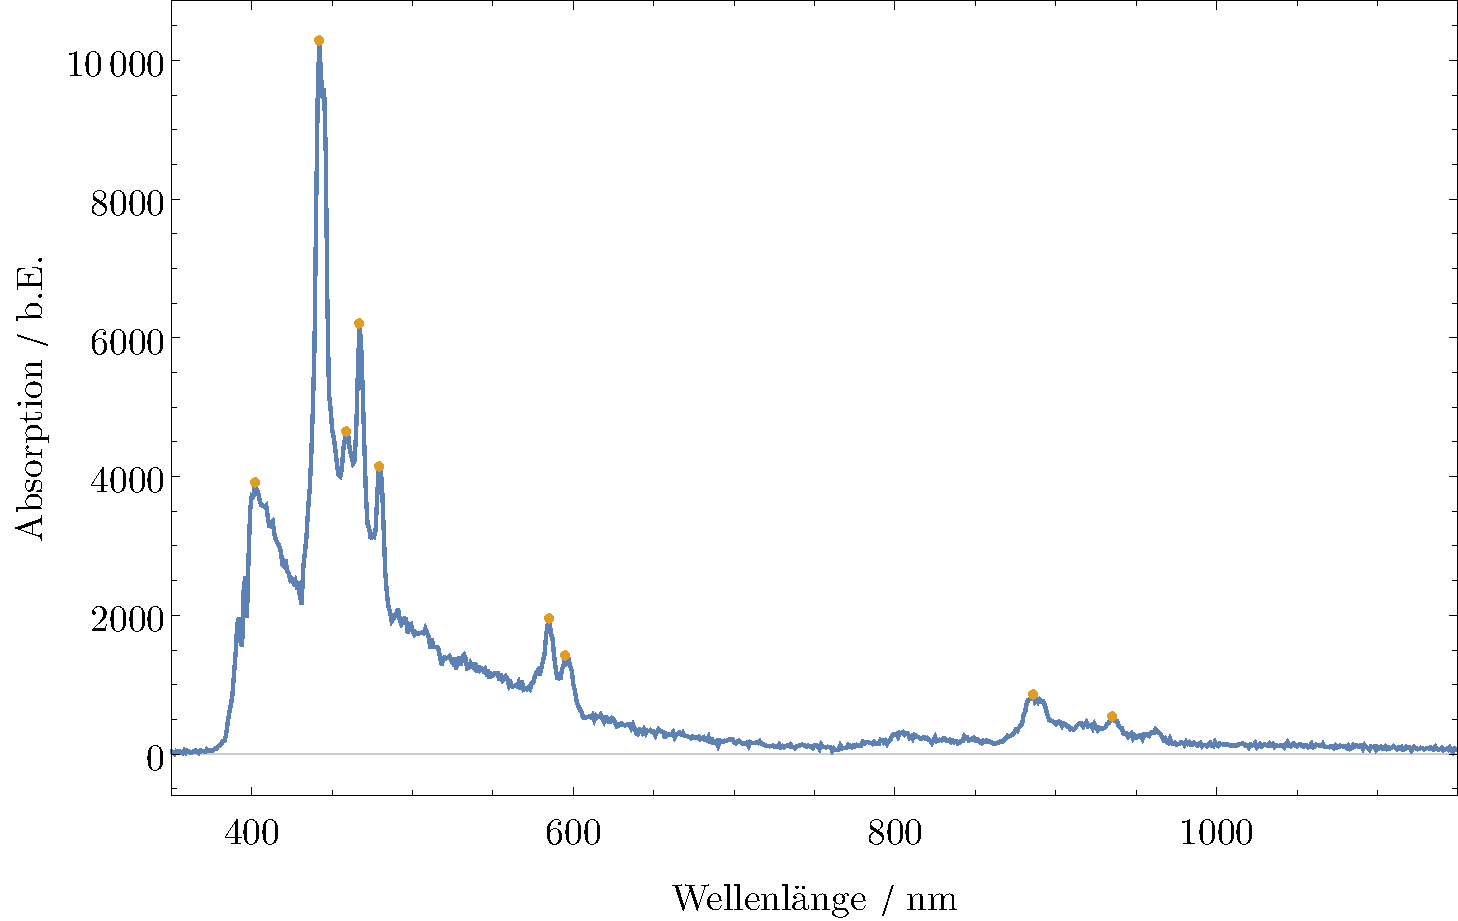
\includegraphics[width=\textwidth]{AbsSpec.pdf}
  \caption{Absorptionsspektrum des Pr:YLF-Kristalls und Position der deutlichen Maxima.}
  \label{img:AbsSpec}
\end{center}
\end{figure}

\begin{table}[htb]
\caption{Positionen und relative Intensitäten der Absorptionsmaxima im Spektrum des
Pr:YLF-Kristalls.}
\begin{center}
\begin{tabular}{|c|c|}
\hline
Wellenlänge / nm & Absorption / b.E. \\ \hline
402 & 3918.9 \\ \hline
442 & 10287.3 \\ \hline
459 & 4653.3 \\ \hline
467 & 6203.5 \\ \hline
479 & 4147.4 \\ \hline
585 & 1947.5 \\ \hline
595 & 1420.8 \\ \hline
886 & 850.9 \\ \hline
935 & 535.6 \\ \hline
\end{tabular}
\end{center}
\label{tab:AbsSpec}
\end{table}


\subsubsection{Emissionsspektrum}

\paragraph{Aufbau und Durchführung}
blablabla

\paragraph{Auswertung}

blablabla

\begin{figure}[H]
\begin{center}
  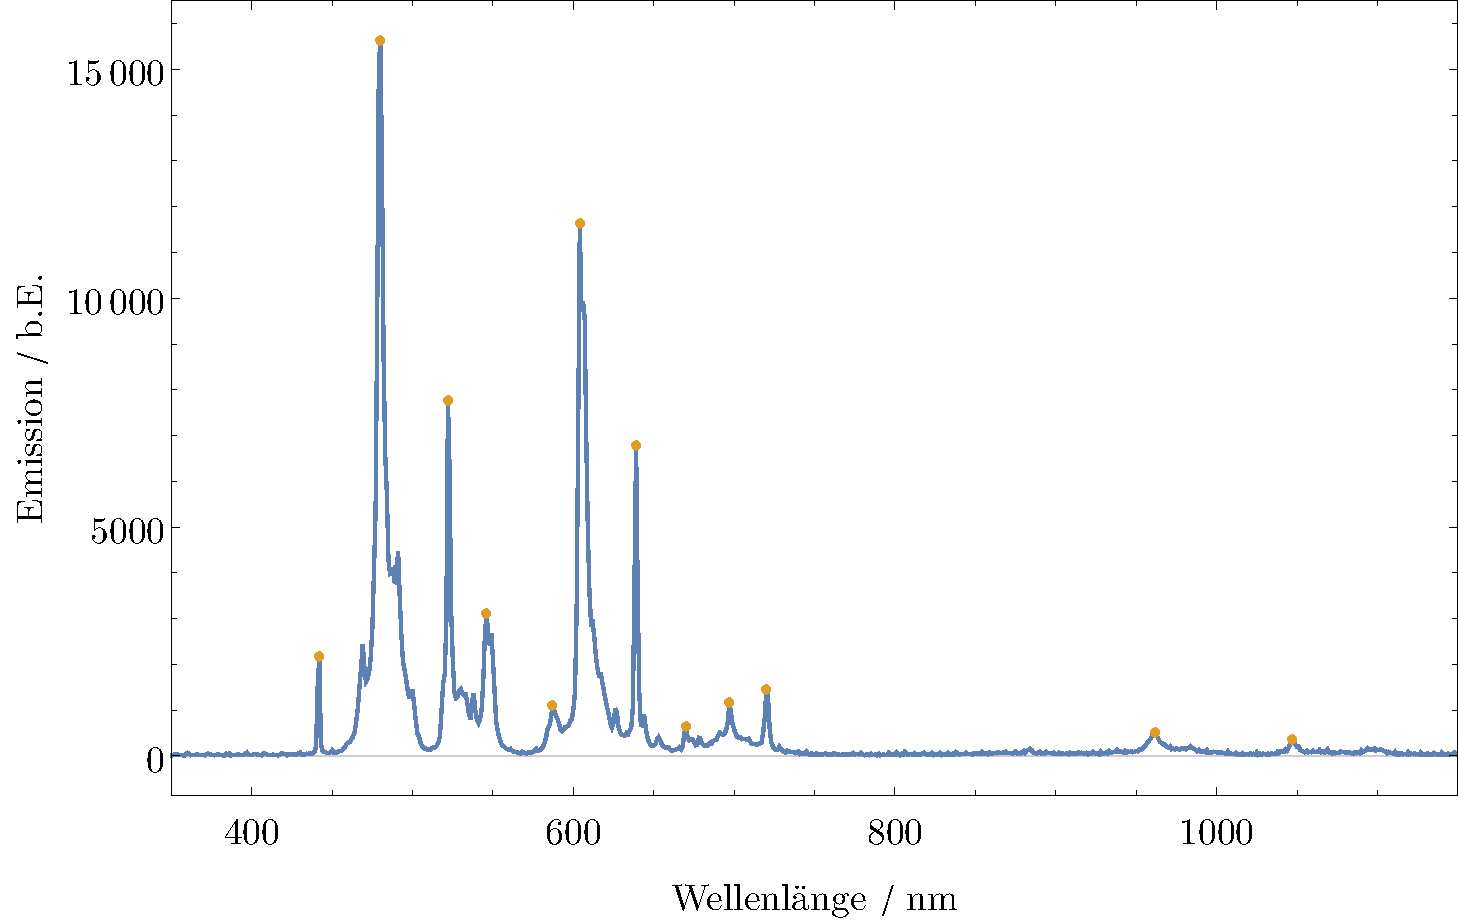
\includegraphics[width=\textwidth]{EmSpec.pdf}
  \caption{Emissionsspektrum des Pr:YLF-Kristalls und Position der deutlichen Maxima.}
  \label{img:EmSpec}
\end{center}
\end{figure}

\begin{table}[htb]
\caption{Positionen und relative Intensitäten der Emissionsmaxima im Spektrum des
Pr:YLF-Kristalls.}
\begin{center}
\begin{tabular}{|c|c|}
\hline
Wellenlänge / nm & Emission / b.E. \\ \hline
442 & 2168.6 \\ \hline
480 & 15633.9 \\ \hline
522 & 7761.3 \\ \hline
546 & 3115.6 \\ \hline
587 & 1099.0 \\ \hline
604 & 11627.5 \\ \hline
639 & 6787.0 \\ \hline
670 & 635.9 \\ \hline
697 & 1162.8 \\ \hline
720 & 1457.7 \\ \hline
962 & 508.6 \\ \hline
1047 & 366.7 \\ \hline
\end{tabular}
\end{center}
\label{tab:EmSpec}
\end{table}


\FloatBarrier


\subsubsection{Messung der Lebensdauer des angeregten Zustands}

\paragraph{Aufbau und Durchführung}

blabla

\paragraph{Auswertung}
Abb.~\ref{img:Lifetime} zeigt die Modulation der Laserspannung während der Messung und das
dazugehörige Fluoreszenzsignal, das von der Photodiode geliefert wird.
Das Photodiodensignal eines einzelnen Abschaltvorgangs ist auf Abb.~\ref{img:LifetimeFit} zu sehen. 
Als Fehler auf die Diodenspannung wird von der Spannungsauflösung des Oszilloskops
(0,2\,mV) ausgegangen und diese - unter Annahme einer Gleichverteilung der Fehler - durch
$2\sqrt{3}$ geteilt.
Der Fit des Signals erfolgt mit einer exponentiellen Abnahme mit der Zeitkonstanten~$\tau$ und dem
Untergrund~$U$. Das Fitergebnis ist auf Tab.~\ref{tab:Fit_lifetime} zu sehen.


\begin{figure}[H]
\begin{center}
  \includegraphics[width=.7\textwidth]{lifetime.png}
  \caption{Modulation des Lasers mit einem Rechtecksignal (gelb) zur Bestimmung der Lebensdauer der
  Fluoreszenz (blau, Messung als Spannungssignal der Photodiode).}
  \label{img:Lifetime}
\end{center}
\end{figure}


\begin{figure}[H]
\begin{center}
  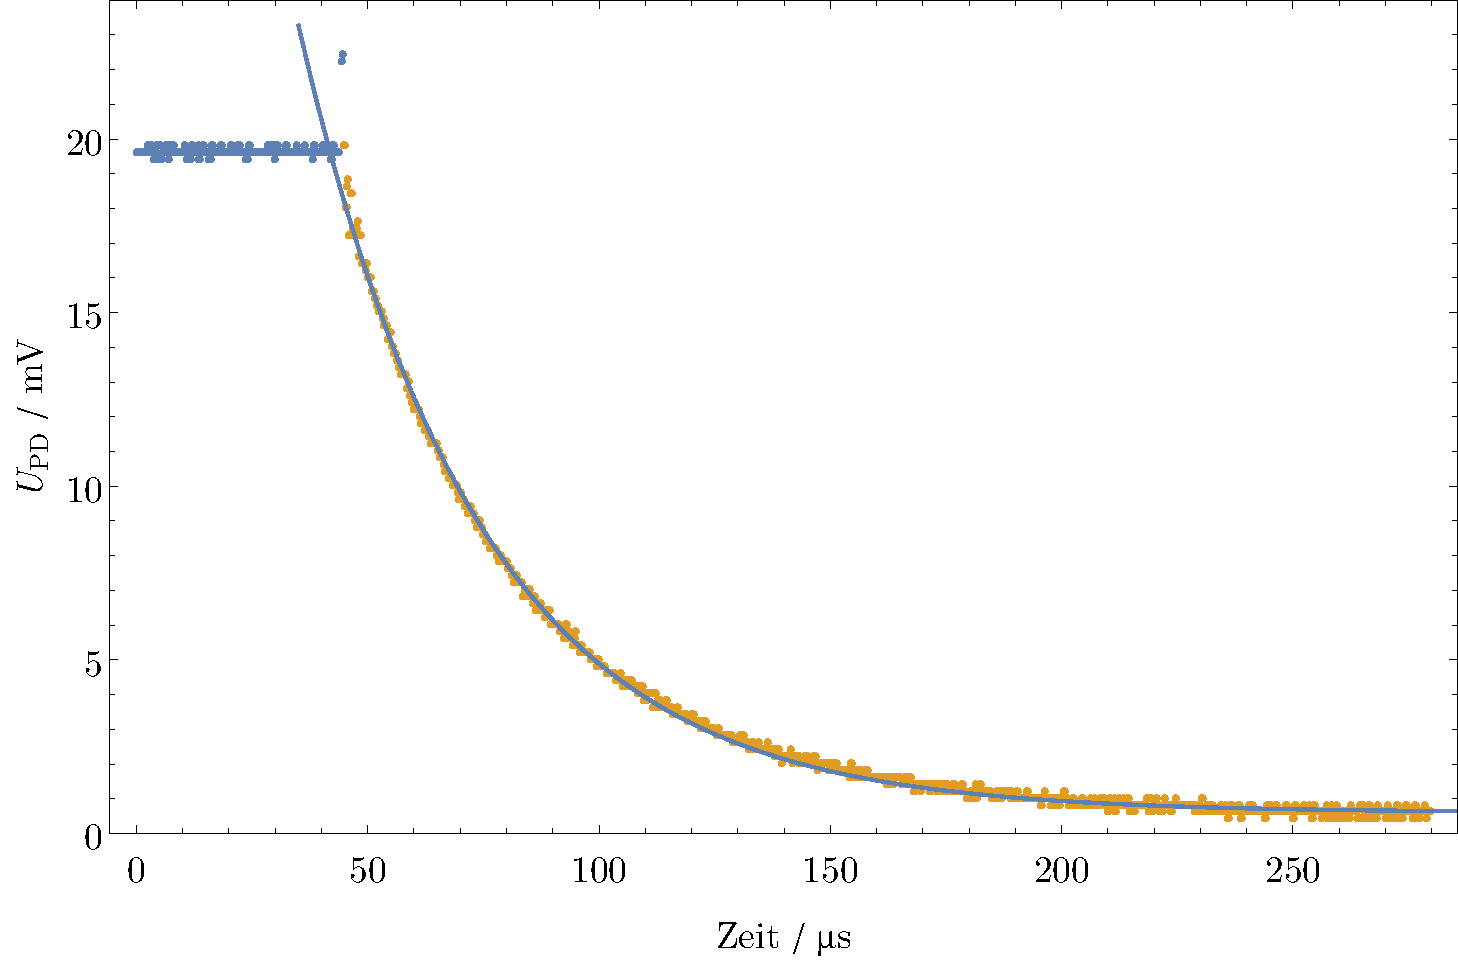
\includegraphics[width=.9\textwidth]{lifetime.pdf}
  \caption{Exponentieller Fit des Spannungssignals der Photodiode $U_{\text{PD}}$ zur Bestimmung der
  Lebenszeit des angeregten Zustands. Der Fitbereich ist gelb markiert, auf die Darstellung der geringen Fehler
  wurde verzichtet.}
  \label{img:LifetimeFit}
\end{center}
\end{figure}

\begin{table}[htb]
\caption{Ergebnisse des Fits der Fluoreszenzlebensdauer mit
$y=A\,\exp(-x/\tau)\,+\,U$.}
\begin{center}
\begin{tabular}{|c|c|}
\hline
$A$ & 55.65\,$\pm$\,0.21\,mV \\ \hline
$\tau$ & 39.01\,$\pm$\,0.10\,\textmu s \\ \hline
$U$ & 0.605\,$\pm$\,0.008\,mV \\ \hline
\textchi$^2$ & 527.875 \\ \hline
\textchi$^2$/\,DoF & 0.450021 \\ \hline
\end{tabular}
\end{center}
\label{tab:Fit_lifetime}
\end{table}


\subsubsection{Messung der absorbierten Leistung}

\paragraph{Aufbau und Durchführung}
blabla

\paragraph{Auswertung}
blabla
 
\begin{table}[htb]
\caption{Leistung am Leistungsmesskopf ohne Kristall im Strahlengang ($P_\text{ohne}$),
mit Kristall ($P_\text{mit}$), absorbierte Leistung ($P_\text{abs}$) und relative Absorption
$P_\text{abs}/P_\text{ohne}$ in Abhängigkeit von Lasertemperatur $T$ und Laserstrom $I$.}
\begin{center}
\begin{tabular}{|c|c|c|c|c|c|}
\hline
T / \grad & I / mA & $P_\text{mit}$ / mW & $P_\text{ohne}$ / mW & $P_\text{abs}$ / mW & Absorption / \% \\ \hline
25 & 400 & 114 & 427 & 313 & 73.3 \\ \hline
25 & 600 & 149 & 737 & 588 & 79.8 \\ \hline
25 & 800 & 87.4 & 532 & 444.6 & 83.6 \\ \hline
35 & 400 & 77.1 & 408 & 330.9 & 81.1 \\ \hline
35 & 600 & 105 & 718 & 613 & 85.4 \\ \hline
35 & 800 & 30.6 & 522 & 491.4 & 94.1 \\ \hline
\end{tabular}
\end{center}
\label{tab:Absorption}
\end{table}
